\begin{frame}{Regression SR: Transformers, Then Mamba}
  \begin{columns}[T,onlytextwidth]
    \column{0.53\textwidth}
      \begin{itemize}\footnotesize\itemsep0.3em
        \item \textbf{Pixel shuffle} (depth-to-space) upsamples once, at the end: a convolution outputs $C r^2$ channels at low resolution, which are rearranged into an $rH \times rW \times C$ image.
        \item \textbf{SwinIR} (2021) stacks shifted-window attention with convolutions. \textbf{HAT} (2023) adds channel attention (each feature channel reweighted by a learned global score) and overlapping cross-attention, so each output pixel draws on more input pixels.
        \item \textbf{Mamba} layers (selective state-space models) run a recurrence over the token sequence in linear time:
        \[ h_k = \bar{A} h_{k-1} + \bar{B} x_k, \qquad y_k = C h_k \]
        $x_k$ is the $k$-th token, $h_k$ a hidden state, $y_k$ the output (plus a skip term); $\bar{B}$, $C$ and the step size inside $\bar{A}$ are computed from the input. \textbf{MambaIR} (2024) scans the image in four directions; \textbf{MambaIRv2} (2025) needs one scan.
      \end{itemize}
    \column{0.45\textwidth}
      {\centering\scriptsize\setlength{\tabcolsep}{4pt}
      \begin{tabular}{l c c c}
        \toprule
        \textbf{Model} & \textbf{Params} & \textbf{Urban100} & \textbf{Manga109} \\
        \midrule
        SwinIR & 11.9M & 27.45 & 32.03 \\
        HAT & 20.8M & 27.97 & 32.48 \\
        MambaIR & 20.4M & 27.68 & 32.32 \\
        MambaIRv2-B & 23.1M & 27.89 & 32.57 \\
        MambaIRv2-L & 34.2M & \textbf{28.07} & \textbf{32.66} \\
        \bottomrule
      \end{tabular}\par}
      \vspace{0.2em}
      {\scriptsize $\times 4$ PSNR (dB, Y channel), bicubic inputs, trained on DF2K (DIV2K plus Flickr2K). Guo et al., ``MambaIRv2: Attentive State Space Restoration,'' CVPR 2025, \href{https://arxiv.org/abs/2411.15269v2}{arXiv:2411.15269v2}, Table~4.\par}
      \vspace{0.4em}
      \begin{itemize}\footnotesize\itemsep0.3em
        \item Four years bought $+0.62$\,dB on Urban100, with about $3\times$ the parameters.
        \item Trained with pixel losses, these models still smooth away texture on real photos: they sit at the low-distortion end of the trade-off.
      \end{itemize}
  \end{columns}
\end{frame}

\begin{frame}{Diffusion Priors for Real-World SR}
  \centering
  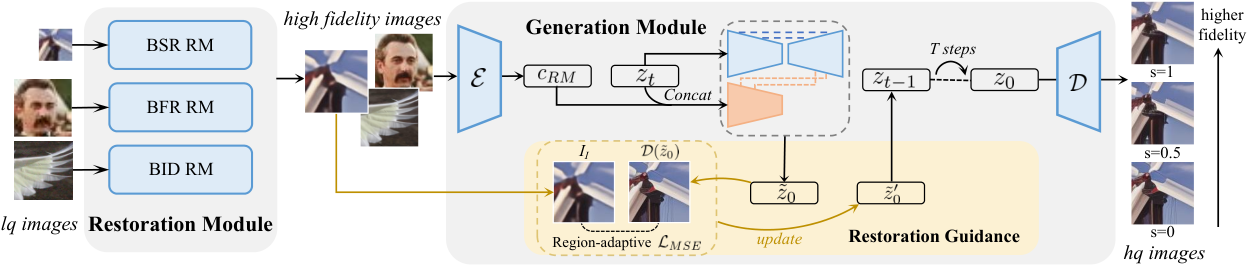
\includegraphics[width=\textwidth,height=0.17\textheight,keepaspectratio]{images/image-restoration-applications/diffbir_fig3_two_stage_pipeline.png}\\[0.1em]
  {\scriptsize Lin et al., ``DiffBIR: Towards Blind Image Restoration with Generative Diffusion Prior,'' ECCV 2024, \href{https://arxiv.org/abs/2308.15070v3}{arXiv:2308.15070v3}, Figure~3.\par}
  \begin{itemize}\footnotesize\itemsep0.2em
    \item A pretrained text-to-image diffusion model already knows what natural textures look like; the restorer only learns to steer it with the low-quality (LQ) input.
    \item \textbf{StableSR} (IJCV 2024) keeps Stable Diffusion (SD) frozen and trains a time-aware encoder that modulates it; one scalar in a feature-wrapping module trades quality for fidelity.
    \item \textbf{DiffBIR} (ECCV 2024, above) first removes degradations with a restoration module, then regenerates detail with IRControlNet on a latent diffusion model; the guidance scale $s$ sets fidelity.
    \item \textbf{SeeSR} (CVPR 2024) trains a degradation-aware prompt extractor that reads image tags off the LQ input, so the prior generates the right semantics.
    \item Shared recipe: frozen prior, a trainable conditioning branch (ControlNet in DiffBIR and SeeSR; feature modulation in StableSR), synthetic training pairs, 50 to 200 sampling steps per image.
  \end{itemize}
  {\scriptsize StableSR: \href{https://arxiv.org/abs/2305.07015v4}{arXiv:2305.07015v4}; SeeSR: \href{https://arxiv.org/abs/2311.16518v2}{arXiv:2311.16518v2}.\par}
\end{frame}

\begin{frame}{SUPIR: Scaling Prior, Data and Prompts}
  \centering
  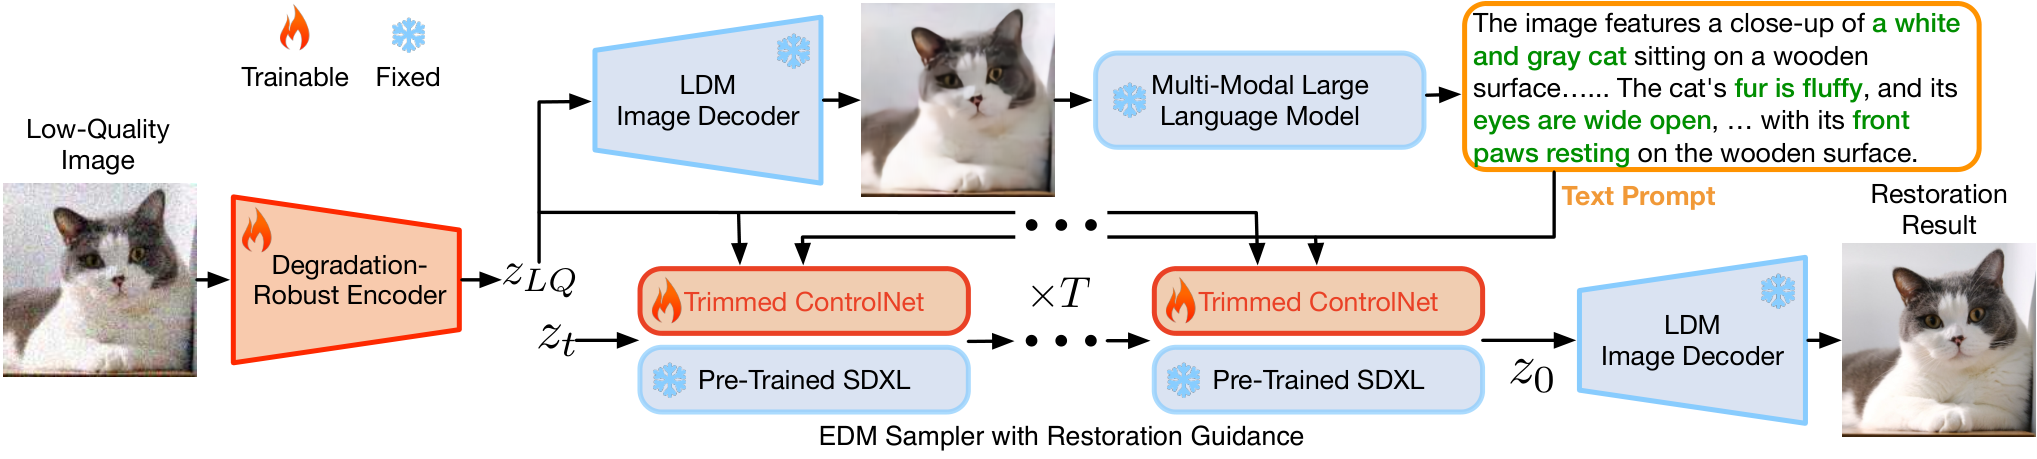
\includegraphics[width=\textwidth,height=0.30\textheight,keepaspectratio]{images/image-restoration-applications/supir_fig2_workflow.png}\\[0.1em]
  {\scriptsize Yu et al., ``Scaling Up to Excellence: Practicing Model Scaling for Photo-Realistic Image Restoration In the Wild,'' CVPR 2024, \href{https://arxiv.org/abs/2401.13627v2}{arXiv:2401.13627v2}, Figure~2; memory and licence: \href{https://github.com/Fanghua-Yu/SUPIR}{github.com/Fanghua-Yu/SUPIR}.\par}
  \vspace{0.2em}
  \begin{columns}[T,onlytextwidth]
    \column{0.49\textwidth}
      \begin{itemize}\footnotesize\itemsep0.3em
        \item \textbf{Prior:} frozen SDXL (2.6B parameters). Trained parts: a degradation-robust encoder and a trimmed ControlNet, joined to SDXL by ZeroSFT connectors (zero-initialised convolutions plus feature modulation).
        \item \textbf{Data:} 20M high-quality $1024 \times 1024$ images with text annotations, plus 70K faces. At test time LLaVA-v1.5-13B captions the decoded LQ input.
        \item \textbf{Cost:} 10 days on 64 A6000 GPUs.
      \end{itemize}
    \column{0.49\textwidth}
      \begin{itemize}\footnotesize\itemsep0.3em
        \item \textbf{Negative-quality prompts} via CFG (``oil painting, cartoon, blur, dirty, messy, low quality, \ldots''); 100K SDXL-generated bad images join the training set so the model learns what they mean.
        \item \textbf{Restoration-guided sampling} pulls each step toward the LQ latent with weight $k_t = (t/T)^r$: strong early for structure, weak late for texture.
        \item The low-memory mode still needs 12\,GB of GPU memory for diffusion plus 16\,GB for LLaVA; non-commercial licence.
      \end{itemize}
  \end{columns}
\end{frame}

\begin{frame}{One-Step Diffusion SR: OSEDiff}
  \begin{columns}[T,onlytextwidth]
    \column{0.53\textwidth}
      \begin{itemize}\footnotesize\itemsep0.3em
        \item Start from the LQ latent instead of noise and denoise \textbf{once}: $\hat{x} = \mathcal{D}\big(F_\theta(\mathcal{E}_\theta(x_L);\, c_y)\big)$, with $\mathcal{E}_\theta$ the VAE encoder plus LoRA, $F_\theta$ one step of a LoRA-tuned SD~2.1 U-Net, $\mathcal{D}$ the frozen decoder, $c_y$ tags read off the LQ image $x_L$.
        \item Loss: MSE $+\,\lambda_1$ LPIPS for fidelity, $+\,\lambda_2$ VSD for realism.
        \item \textbf{Variational score distillation (VSD):} the frozen SD $\epsilon_\phi$ and a LoRA copy $\epsilon_{\phi'}$ trained on the generator's own outputs both denoise the noised output latent $\hat{z}_t$:
        \[ \nabla_\theta \mathcal{L}_{\mathrm{VSD}} = \mathbb{E}_{t,\epsilon}\Big[\omega(t)\big(\epsilon_\phi(\hat{z}_t) - \epsilon_{\phi'}(\hat{z}_t)\big)\frac{\partial \hat{z}_H}{\partial \theta}\Big] \]
        Both denoisers are also conditioned on $t$ and $c_y$; $\omega(t)$ weights timesteps and $\hat{z}_H$ is the output latent. The difference moves outputs from ``what the generator makes'' toward ``what the prior expects'', a KL-divergence objective.
      \end{itemize}
    \column{0.45\textwidth}
      {\centering\scriptsize\setlength{\tabcolsep}{3pt}
      \begin{tabular}{l c c c}
        \toprule
        \textbf{Method} & \textbf{Steps} & \textbf{Time (s)} & \textbf{Trainable (M)} \\
        \midrule
        StableSR & 200 & 11.50 & 150.0 \\
        DiffBIR & 50 & 2.72 & 380.0 \\
        SeeSR & 50 & 4.30 & 749.9 \\
        ResShift & 15 & 0.71 & 118.6 \\
        SinSR & 1 & 0.13 & 118.6 \\
        OSEDiff & 1 & \textbf{0.11} & \textbf{8.5} \\
        \bottomrule
      \end{tabular}\par}
      \vspace{0.2em}
      {\scriptsize $512 \times 512$ input, one A100. Wu et al., ``One-Step Effective Diffusion Network for Real-World Image Super-Resolution,'' NeurIPS 2024, \href{https://arxiv.org/abs/2406.08177v3}{arXiv:2406.08177v3}, Table~2.\par}
      \vspace{0.3em}
      \begin{itemize}\scriptsize\itemsep0.25em
        \item ResShift (NeurIPS 2023) diffuses between the low-resolution (LR) and high-resolution (HR) images by shifting their residual, in 15 steps; SinSR (CVPR 2024) distils it into one.
        \item OSEDiff trains in about a day on 4 A100 GPUs; code is Apache-2.0.
      \end{itemize}
  \end{columns}
\end{frame}

\begin{frame}{Frontier: Transformer Priors and Fewer Steps}
  \footnotesize
  Since 2024, restorers adopt larger priors, often diffusion transformers (DiT), and keep cutting the number of steps.\par
  \vspace{0.3em}
  {\centering\scriptsize
  \begin{tabular}{>{\raggedright\arraybackslash}p{1.45cm} >{\raggedright\arraybackslash}p{1.65cm} >{\raggedright\arraybackslash}p{2.15cm} >{\raggedright\arraybackslash}p{6.4cm}}
    \toprule
    \textbf{Model} & \textbf{Venue} & \textbf{Prior} & \textbf{Key idea} \\
    \midrule
    InvSR & CVPR 2025 & SD-Turbo & a noise predictor maps the LR image to an intermediate diffusion state; 1 to 5 sampling steps, chosen per image \\
    \addlinespace[0.15em]
    TSD-SR & CVPR 2025 & SD3 (teacher) & one-step student trained by target score distillation, which adds real-image references; about $40\times$ faster than SeeSR \\
    \addlinespace[0.15em]
    DreamClear & NeurIPS 2024 & PixArt-$\alpha$ (DiT) & 1M privacy-safe synthetic training images; a per-token mixture of restoration experts; 50 steps \\
    \addlinespace[0.15em]
    DiT4SR & ICCV 2025 & SD3 (MM-DiT) & the LR latent joins joint attention as its own token stream and evolves with the sample \\
    \addlinespace[0.15em]
    LucidFlux & ICLR 2026 & FLUX.1 (12B) & caption-free: SigLIP features of a lightly restored proxy replace text prompts; 28 steps \\
    \bottomrule
  \end{tabular}\par}
  \vspace{0.3em}
  \begin{itemize}\footnotesize\itemsep0.25em
    \item The data recipe did not change: all five train on Real-ESRGAN synthetic pairs. InvSR (S-Lab licence) and LucidFlux (FLUX.1 [dev] licence) are non-commercial.
  \end{itemize}
  {\scriptsize Yue et al., \href{https://arxiv.org/abs/2412.09013v2}{arXiv:2412.09013v2}; Dong et al., \href{https://arxiv.org/abs/2411.18263v4}{arXiv:2411.18263v4}; Ai et al., \href{https://arxiv.org/abs/2410.18666v2}{arXiv:2410.18666v2}; Duan et al., \href{https://arxiv.org/abs/2503.23580v2}{arXiv:2503.23580v2}; Fei et al., \href{https://arxiv.org/abs/2509.22414v4}{arXiv:2509.22414v4}.\par}
\end{frame}

\begin{frame}{Super-Resolution on a Phone: NTIRE 2026}
  \begin{columns}[T,onlytextwidth]
    \column{0.46\textwidth}
      \begin{itemize}\footnotesize\itemsep0.35em
        \item The NTIRE 2026 challenge (New Trends in Image Restoration and Enhancement, a CVPR 2026 workshop) asked for $\times 4$ real-world SR under a phone budget: $128 \times 128$ inputs, timed at 16-bit precision on a MediaTek Dimensity 8400 chip.
        \item Ranking $= 2^{\,\text{perceptual}} \times \text{speedup}^{0.2}$. The perceptual score adds six IQA terms (LPIPS, DISTS, CLIP-IQA, MANIQA, MUSIQ, NIQE); speedup is measured against OSEDiff on the same chip.
        \item 108 registrants, 16 valid final entries. One-step diffusion with LoRA was the usual starting point, and distillation was needed to fit the phone.
      \end{itemize}
    \column{0.52\textwidth}
      {\centering\scriptsize\setlength{\tabcolsep}{3pt}
      \begin{tabular}{c >{\raggedright\arraybackslash}p{2.9cm} c c}
        \toprule
        \textbf{Rank} & \textbf{Approach} & \textbf{Perc.} & \textbf{Speedup} \\
        \midrule
        1 & compact CNN, fine-tuned on IQA metrics & 4.03 & $113.85\times$ \\
        2 & Real-ESRGAN generator fine-tuned with IQA losses & 4.17 & $21.79\times$ \\
        3 & OSEDiff distilled into a pruned U-Net and a tiny decoder & 4.24 & $11.67\times$ \\
        4 & one-step latent diffusion & \textbf{4.35} & $1.00\times$ \\
        \bottomrule
      \end{tabular}\par}
      \vspace{0.2em}
      {\scriptsize Li et al., ``The First Challenge on Mobile Real-World Image Super-Resolution at NTIRE 2026: Benchmark Results and Method Overview,'' NTIRE 2026 report, \href{https://arxiv.org/abs/2604.17306}{arXiv:2604.17306}, Table~1, Eqs.~1--3, Secs.~3.4 and 4.1--4.4.\par}
      \vspace{0.3em}
      \begin{itemize}\footnotesize
        \item Small convolutional networks tuned on IQA metrics won the combined score; the best perceptual score still came from one-step diffusion.
      \end{itemize}
  \end{columns}
\end{frame}

\begin{frame}{Video SR: Consistent Detail Across Frames}
  \centering
  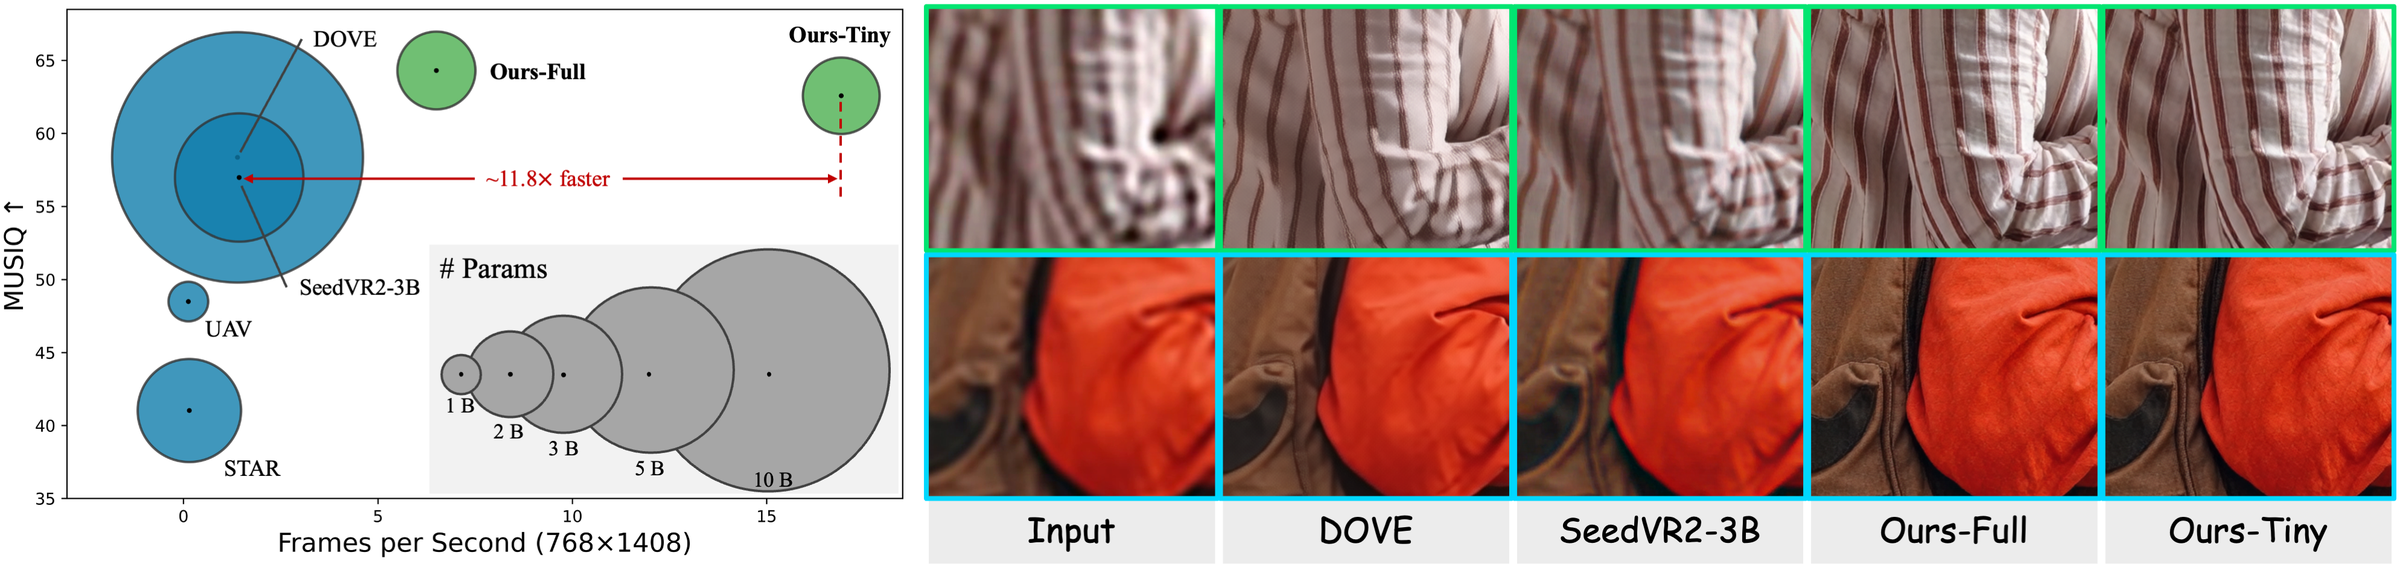
\includegraphics[width=\textwidth,height=0.29\textheight,keepaspectratio]{images/image-restoration-applications/flashvsr_fig1_speed_quality.png}\\[0.1em]
  {\scriptsize MUSIQ against frames per second (FPS) at $768 \times 1408$; bubble size shows parameter count. Zhuang et al., ``FlashVSR: Towards Real-Time Diffusion-Based Streaming Video Super-Resolution,'' CVPR 2026, \href{https://arxiv.org/abs/2510.12747v1}{arXiv:2510.12747v1}, Figure~1 (bottom row).\par}
  \vspace{0.2em}
  \begin{columns}[T,onlytextwidth]
    \column{0.49\textwidth}
      \begin{itemize}\scriptsize\itemsep0.25em
        \item Restoring frames one at a time makes sampled texture flicker; video SR has to be faithful and consistent over time.
        \item \textbf{Upscale-A-Video} (CVPR 2024): temporal layers in the U-Net and VAE decoder keep short clips consistent; training-free, flow-guided propagation of latents covers the whole video.
        \item \textbf{SeedVR} (CVPR 2025): a diffusion transformer with shifted-window attention on a latent compressed $4\times$ in time and $8\times$ in space; any length and resolution.
      \end{itemize}
    \column{0.49\textwidth}
      \begin{itemize}\scriptsize\itemsep0.25em
        \item \textbf{SeedVR2} (ICLR 2026): one step, through adversarial post-training against real videos; 3B and 7B models under Apache-2.0. Its model card warns of over-generated detail on lightly degraded inputs.
        \item \textbf{FlashVSR} (CVPR 2026): one-step and streaming, with locality-constrained sparse attention and a tiny decoder; its Tiny variant runs at about 17 FPS at $768 \times 1408$ on one A100, roughly $12\times$ faster than SeedVR2-3B; Apache-2.0.
      \end{itemize}
  \end{columns}
  {\scriptsize Zhou et al., \href{https://arxiv.org/abs/2312.06640}{arXiv:2312.06640}; Wang et al., \href{https://arxiv.org/abs/2501.01320v4}{arXiv:2501.01320v4} and \href{https://arxiv.org/abs/2506.05301v2}{arXiv:2506.05301v2}; \href{https://huggingface.co/ByteDance-Seed/SeedVR2-3B}{SeedVR2-3B model card}.\par}
\end{frame}

\begin{frame}{Hallucination: When Generated Detail Is Wrong}
  \begin{columns}[T,onlytextwidth]
    \column{0.50\textwidth}
      \centering
      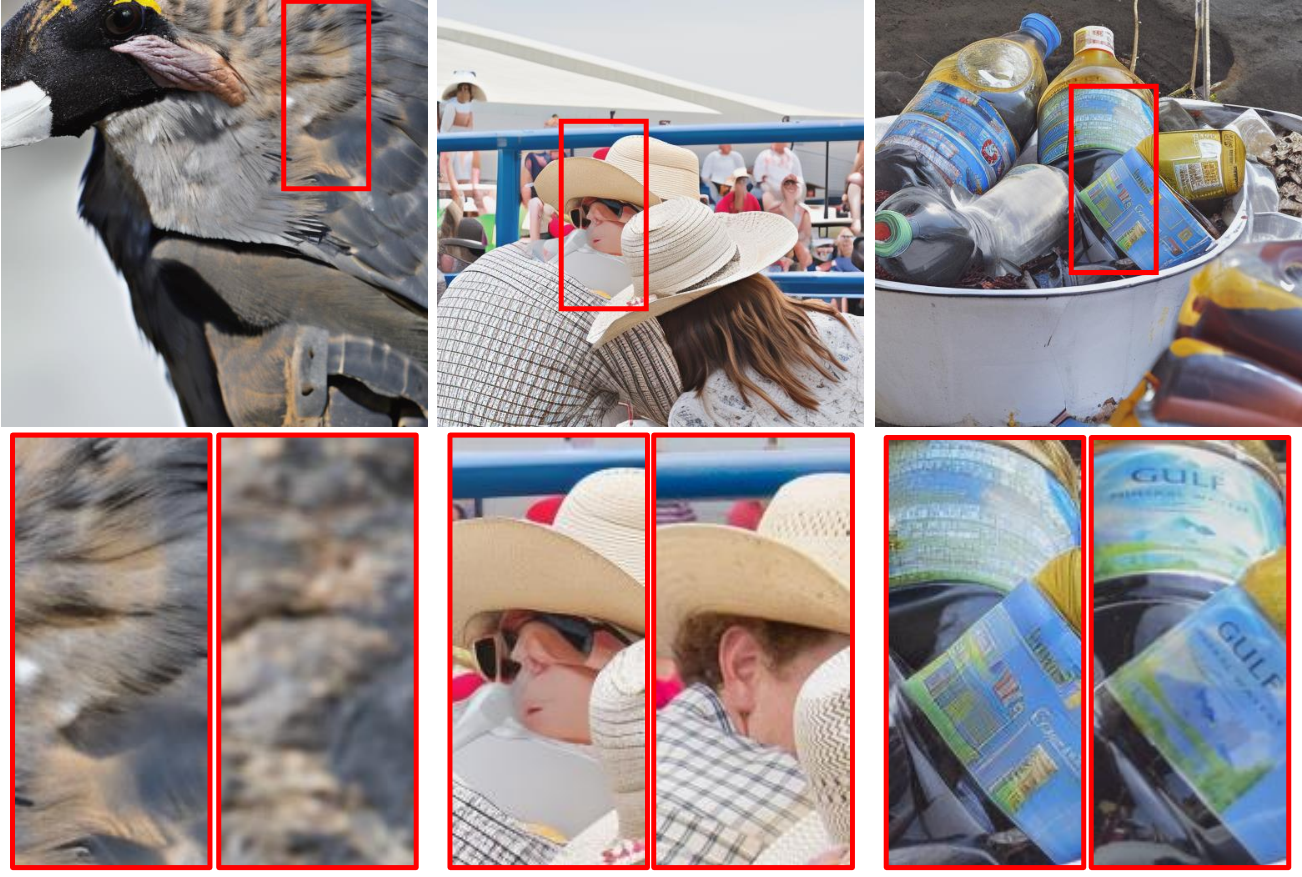
\includegraphics[width=\linewidth,height=0.60\textheight,keepaspectratio]{images/image-restoration-applications/hallucination_score_fig2_examples.png}\\[0.1em]
      {\scriptsize SeeSR outputs (top); zoom-ins of output (left) and ground truth (right) below. Ren et al., ``Hallucination Score: Towards Mitigating Hallucinations in Generative Image Super-Resolution,'' arXiv 2025, \href{https://arxiv.org/abs/2507.14367v2}{arXiv:2507.14367v2}, Figure~2.\par}
    \column{0.48\textwidth}
      \begin{itemize}\footnotesize\itemsep0.35em
        \item A generative restorer samples \emph{one} plausible $x$, and the sample can be wrong in ways a viewer trusts: invented texture, a different face, unreadable text (left).
        \item Ren et al.\ find such errors ``orthogonal to both exact fidelity and no-reference quality'': PSNR, SSIM, LPIPS and MUSIQ often miss them, so they score hallucination by prompting a multimodal LLM.
        \item OSEDiff's authors left SUPIR out of their comparison because ``it tends to generate rich yet excessive details, which are however unfaithful to the input image.''
        \item Where pixels are evidence (medical scans, licence plates, satellite change maps), prefer fidelity-oriented models, keep the input next to the output, and distrust text or faces that appear only after upscaling.
      \end{itemize}
  \end{columns}
\end{frame}
